\section{Lecture 5}
\begin{longtable}{p{4cm}p{15cm}}
Synapse		& 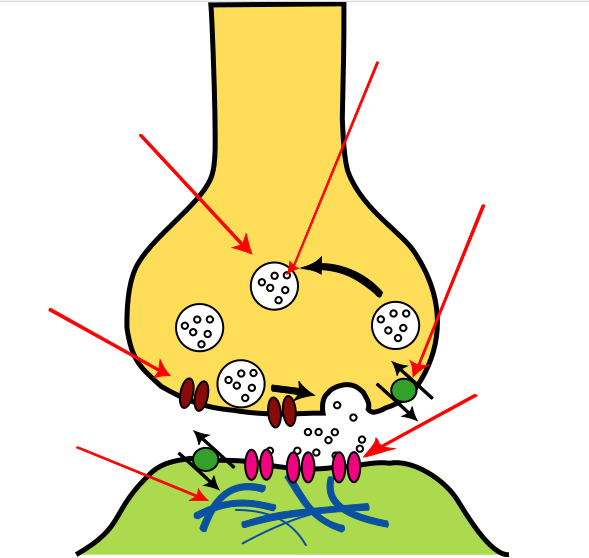
\includegraphics[width = 10cm]{neuroinf_synapse2.png}\\
		& The \textit{synapse} is the cleft between the \textit{presynaptic element} and the \textit{postsynaptic element}.\\
EPSP		& Excitatory postsynaptic potential. Normally, excitatory neurotransmitters open Na$^+$ and K$^+$ channels. Therefore, the conductances for these ions raise, resulting in higher currents, resulting in a change in voltage.\\
IPSP		& Inhibitory postsynaptic potential. Normally, inhibitory neurotransmitters open K$^+$ and Cl$^-$ channels. Therefore, the conductances for these ions raise, resulting in higher currents, resulting in a change in voltage.\\
\textbf{Signal transmission}\\
- At presynaptic element	& \begin{itemize}
                        	  	\item After an \textbf{action potential}, the membrane at the axon terminal is depolarized for a short moment.
					\item Due to the depolarization, voltage-gated \textbf{Ca$^{2+}$-channels} open and Ca$^{2+}$ flows into the presynaptic element.
					\item The increased Ca$^{2+}$ concentration triggers the \textbf{emission of neurotransmitters} into the synaptic cleft.
                        	  \end{itemize}\\
- At postsynaptic element	& \begin{itemize}
                         	  	\item At the postsynaptic element, there are \textbf{ligand-gated ion channels} facing the synapse. The neurotransmitters can ``open'' specific ion channels.
					\item Depending on which ion's channel is opened, an \textbf{EPSP} or \textbf{IPSP} establishes. Mostly, EPSP leads to an increase in membrane voltage, while IPSP mostly lead to a decrease in membrane voltage of the postsynaptic element. Theoretically, EPSP could decrease the membrane voltage, since the channels are opened for both directions
					\item The neurotransmitters are finally removed by enzymes and the membrane voltage levels out again.
                         	  \end{itemize}\\
Electric circuit for synapse	& 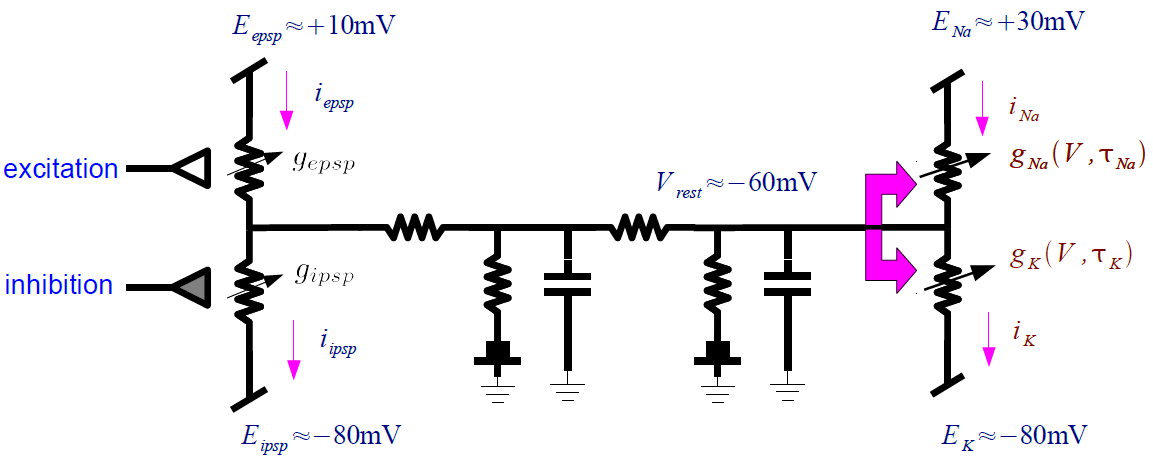
\includegraphics[width = 15cm]{neuroinf_synapse.png}\\
		& The left part is the presynaptic element, the right part is the postsynaptic element. The part in between is in reality repeated many times and represents the leakage.\\
Presynaptic batteries	& $E_{EPSP}$ and $E_{IPSP}$ symbolize the voltages induced by the opening of the ligand-gated ion channels. Therefore, $g_{EPSP}$ and $g_{IPSP}$ depend on ligands (neurotransmitters) and not on voltages. In addition, they are not capable of initiating feedback loops.\\
Postsynaptic batteries	& The already well-known $E_{Na}$ and $E_K$ represent the membrane voltage inside the postsynaptic cell (if their ligand-gated ion channels are closed).\\
Agonist			& An agonist ``enables'' a receptor (of an excitatory or inhibitory ion channel).\\
Antagonist		& An antagonist ``blocks'' a receptor (of an excitatory or inhibitory ion channel).\\
Important neurotransmitter	& \begin{tabular}[t]{ll}
				    Excitatory			& Inhibitory\\\hline
				    Glutamate (always)		& GABA (always except for embryos)\\
				    AMPA (only at specific receptors)\\
				    NMDA (only at specific receptors)\\
				  \end{tabular}\\
\end{longtable}